\chapter{\IfLanguageName{dutch}{Implementatie in Istio}{Implementation in Istio}}
\label{ch:implementatie-backend-istio}

Om de services in Istio te implementeren, moeten we eerst de services definiëren in \textit{YAML}-bestanden. In deze bestanden definiëren we de services, de \textit{VirtualService} en de \textit{Gateway}.

De \textit{Gateway} wordt eenmalig gedefinieerd en definieert de host en de poort waarop de services van buitenaf kunnen worden benaderd. De \textit{VirtualService} definieert de regels voor het routeren van verzoeken naar de services.

Het \textit{Gateway}-bestand zorgt voor het aanmaken van de ingressgateway \ref{fig:gateway}.

De toegestane routeringen worden gedefinieerd in het \textit{VirtualService}-bestand \ref{fig:virtualservice}.

\begin{figure}[H]
    \centering	
    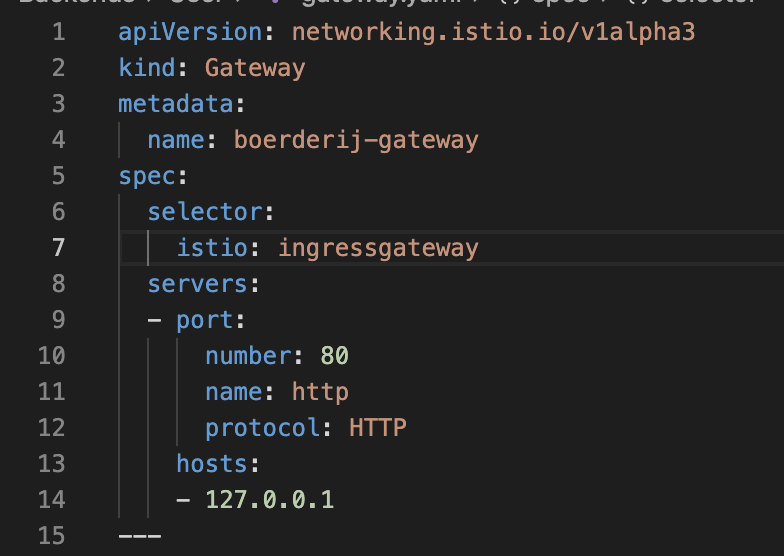
\includegraphics[width = 8cm]{gateway.png} 
    \caption{Voorbeeld van een gateway.yaml bestand} 
    \label{fig:gateway}
\end{figure}

\begin{figure}[H]
    \centering	
    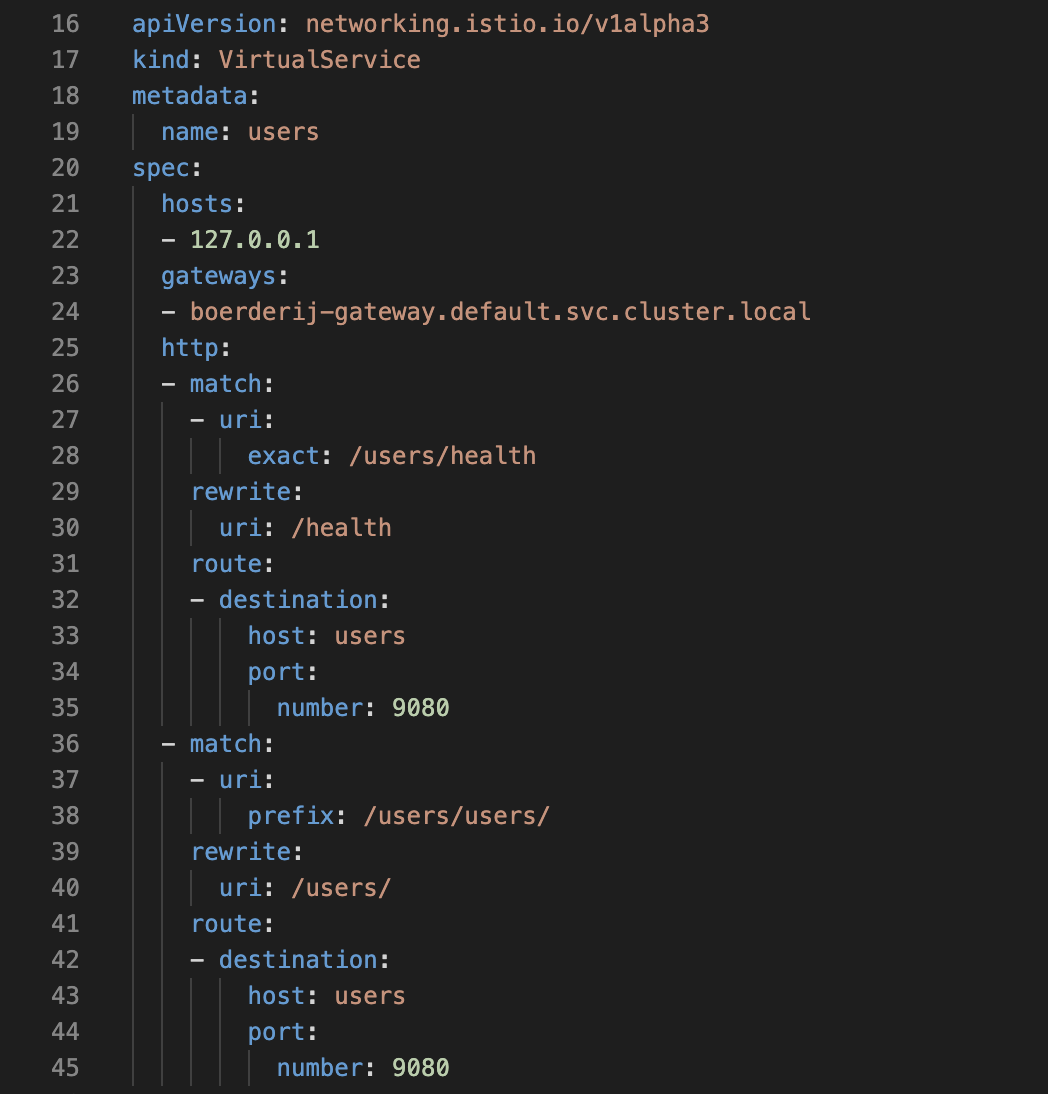
\includegraphics[width = 8cm]{virtualservice.png} 
    \caption{Voorbeeld van een virtualservice.yaml bestand} 
    \label{fig:virtualservice}
\end{figure}

De services blijven draaien in Docker-containers. De containers worden gebouwd met behulp van de Dockerfiles die in de vorige hoofdstukken zijn gemaakt. De containers worden vervolgens gedistribueerd naar een Kubernetes-cluster.

Voor het deployen van de services in Kubernetes, maken we gebruik van \textit{DeploymentYAML}-bestanden. In deze bestanden definiëren we de services, de \textit{Deployment} en de \textit{Service}. De \textit{Deployment} definieert de configuratie van de pod en de \textit{Service} definieert de configuratie van de service.

Binnen Istio krijgt elke service pod naast de applicatie container ook een \textit{sidecar} container. Deze \textit{sidecar} container is verantwoordelijk voor het routeren van het netwerkverkeer naar de applicatie container. De \textit{sidecar} container wordt automatisch toegevoegd door Istio.

Een voorbeeld van een \textit{DeploymentYAML}-bestand is te zien in figuur \ref{fig:deployment}.

\begin{figure}[H]
    \centering	
    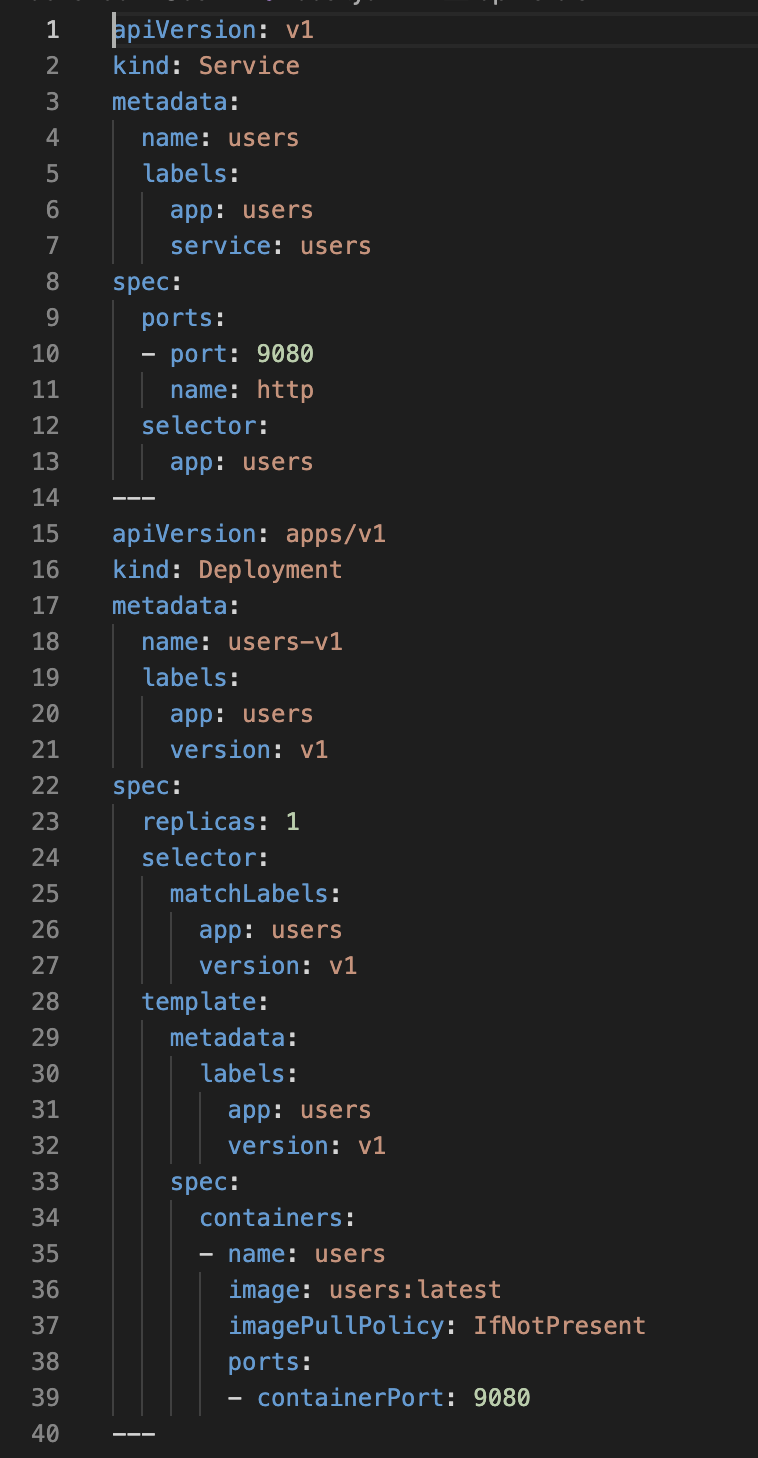
\includegraphics[width = 8cm]{deployment.png} 
    \caption{Voorbeeld van een deployment.yaml bestand} 
    \label{fig:deployment}
\end{figure}

De Kubernetes cluster draait binnen een Minikube Docker container. Om deze lokaal beschikbaar te maken, moet de Minikube tunnel worden gestart. De Minikube tunnel zorgt ervoor dat de services van buitenaf kunnen worden benaderd.

Zodra de services zijn geïmplementeerd in Istio, kunnen we de applicatie benaderen via de gateway-URL. De gateway-URL is de host en poort die is gedefinieerd in het \textit{Gateway}-bestand. De gateway-URL kan worden verkregen door de omgevingsvariabelen \textit{INGRESS\_HOST} en \textit{INGRESS\_PORT} in te stellen. Met behulp van deze omgevingsvariabelen kunnen we de gateway-URL berekenen en de applicatie benaderen via de browser.

Het Kiali-dashboard kan worden geopend met het \textit{istioctl dashboard kiali} commando. Het Kiali-dashboard geeft een visuele weergave van de interacties tussen de verschillende services. Hiermee kunnen we de verkeersstromen en de prestaties van de services monitoren en analyseren.

Wanneer er geen verkeer is, ziet het Kiali-dashboard eruit zoals in figuur \ref{fig:kaili}.
\begin{figure}[H]
    \centering	
    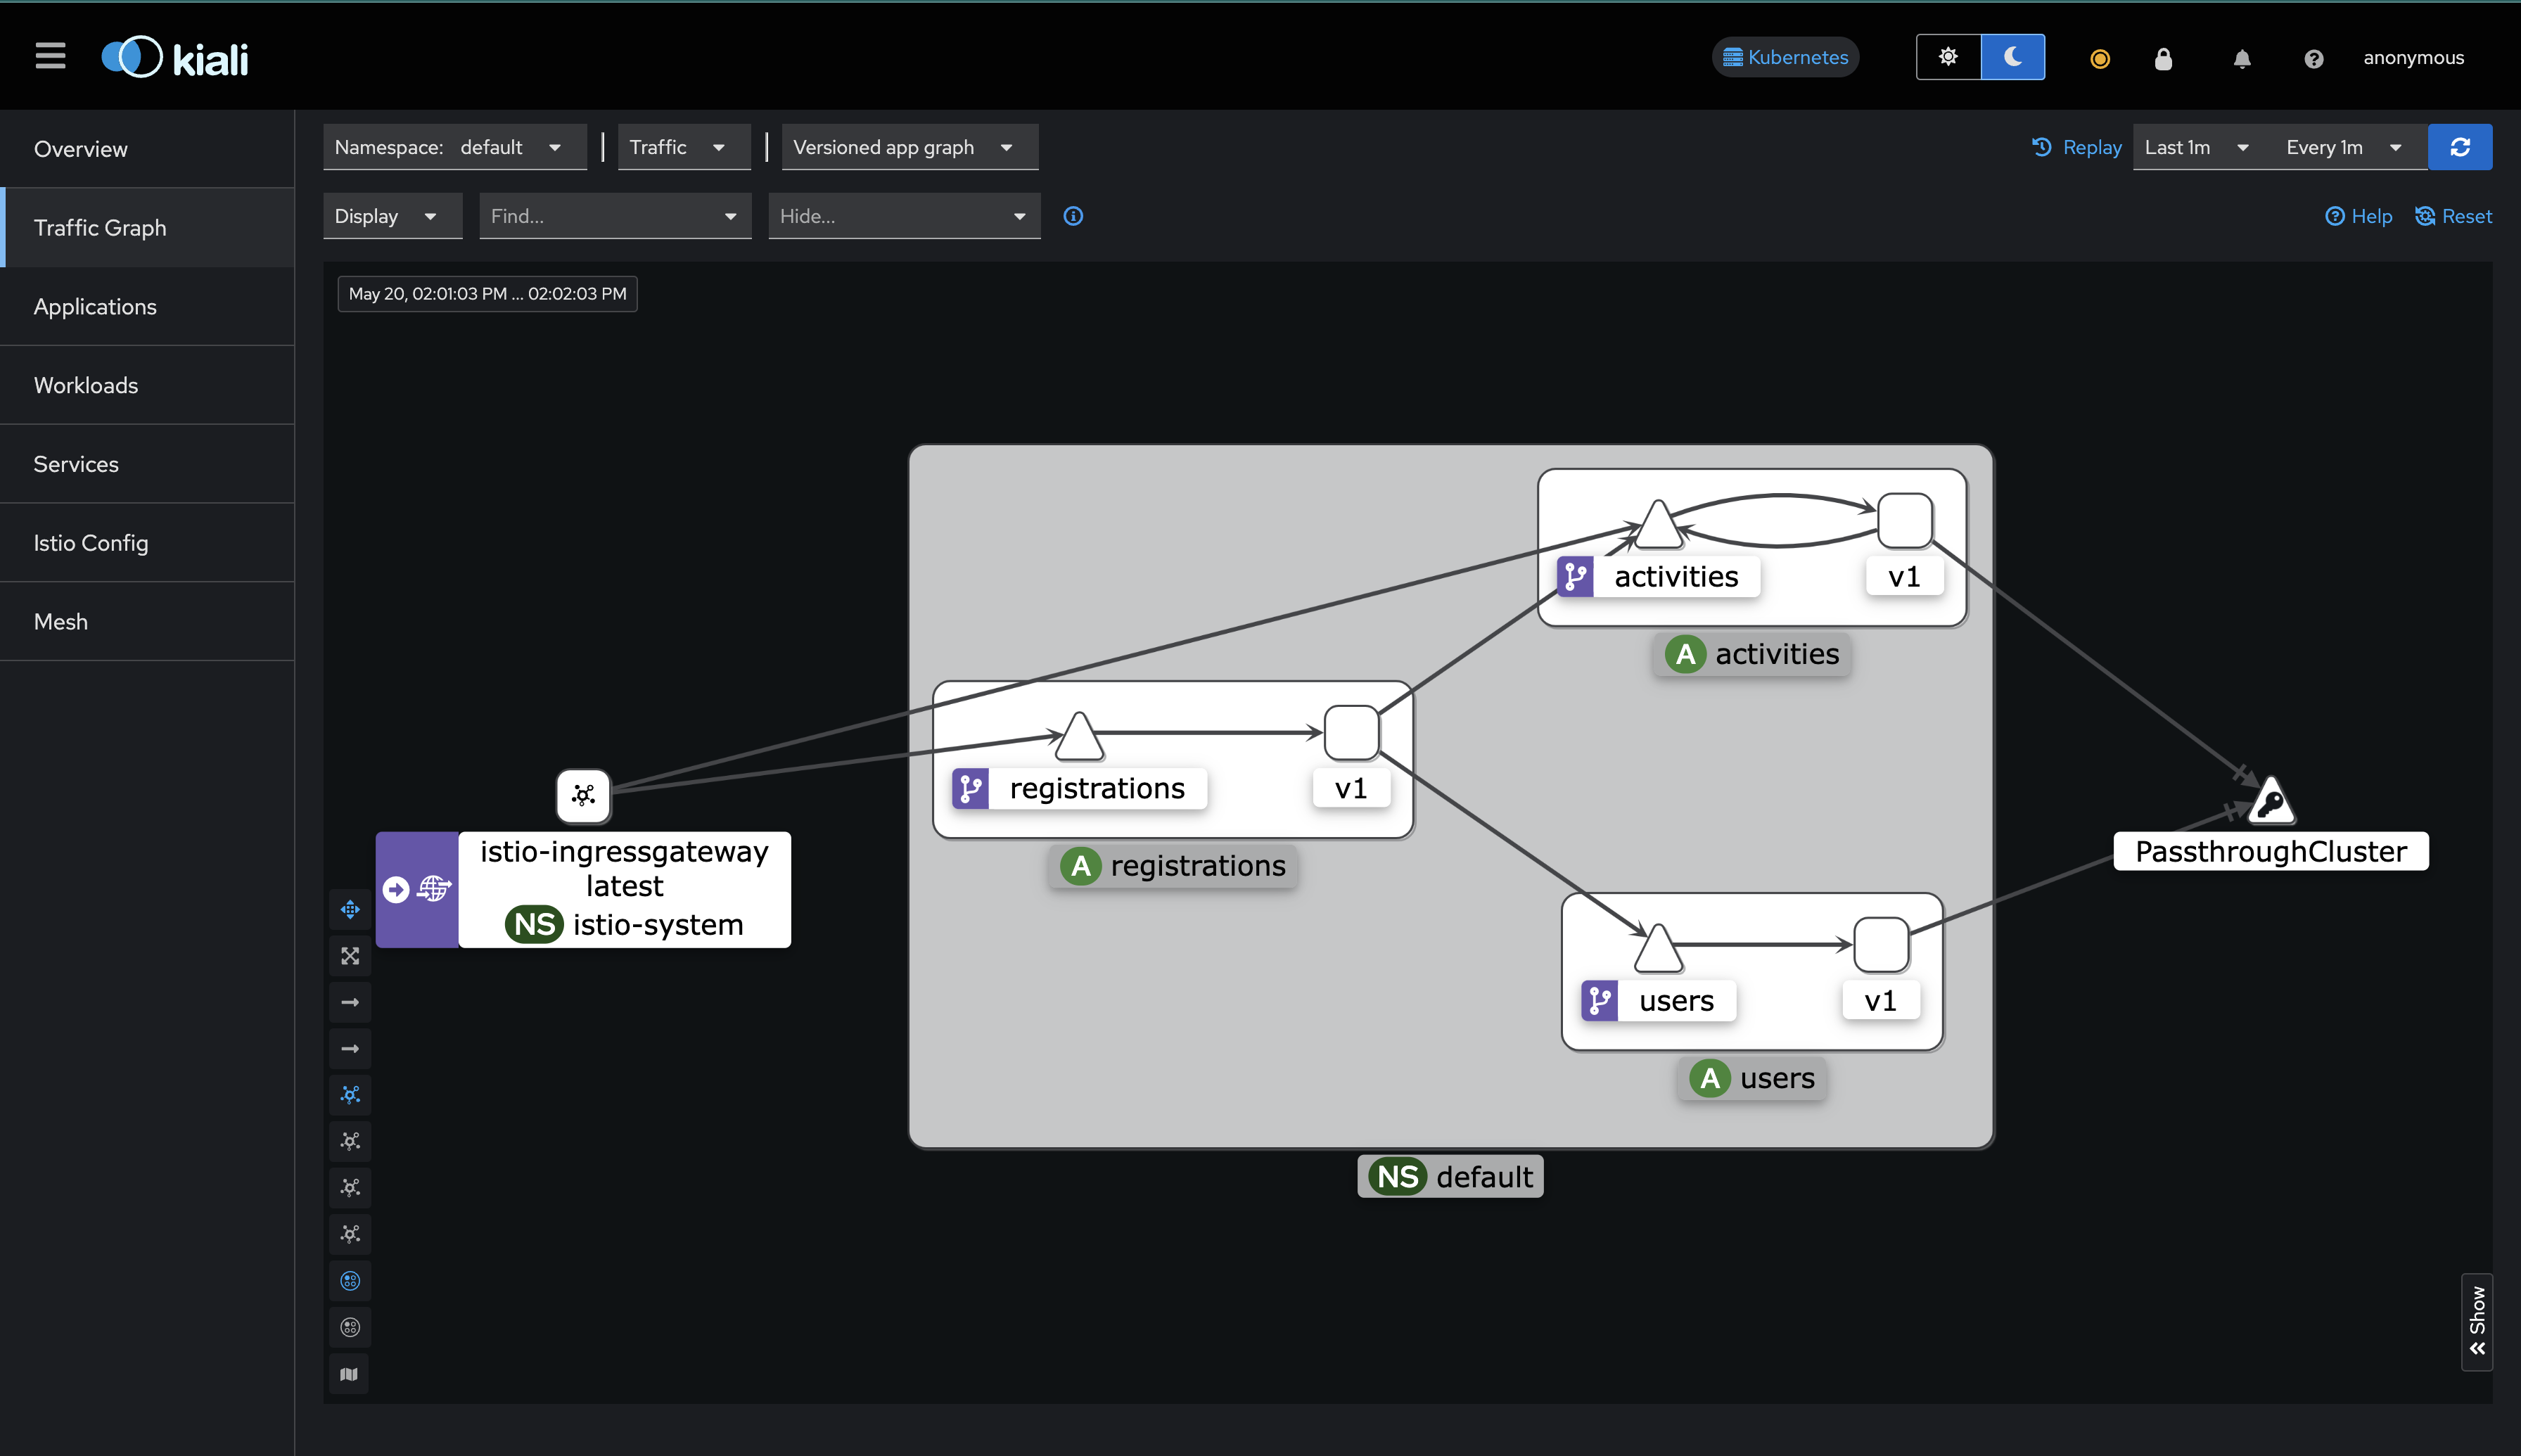
\includegraphics[width = 16cm]{kiali.png} 
    \caption{Kiali Console} 
    \label{fig:kaili}
\end{figure}

Als de activiteitenservice wordt aangeroepen, wordt deze rechtstreeks via de ingressgateway aangeroepen. In de Kiali-console wordt dit weergegeven als een directe verbinding tussen de ingressgateway en de activiteitenservice \ref{fig:kaili2}.

\begin{figure}[H]
    \centering	
    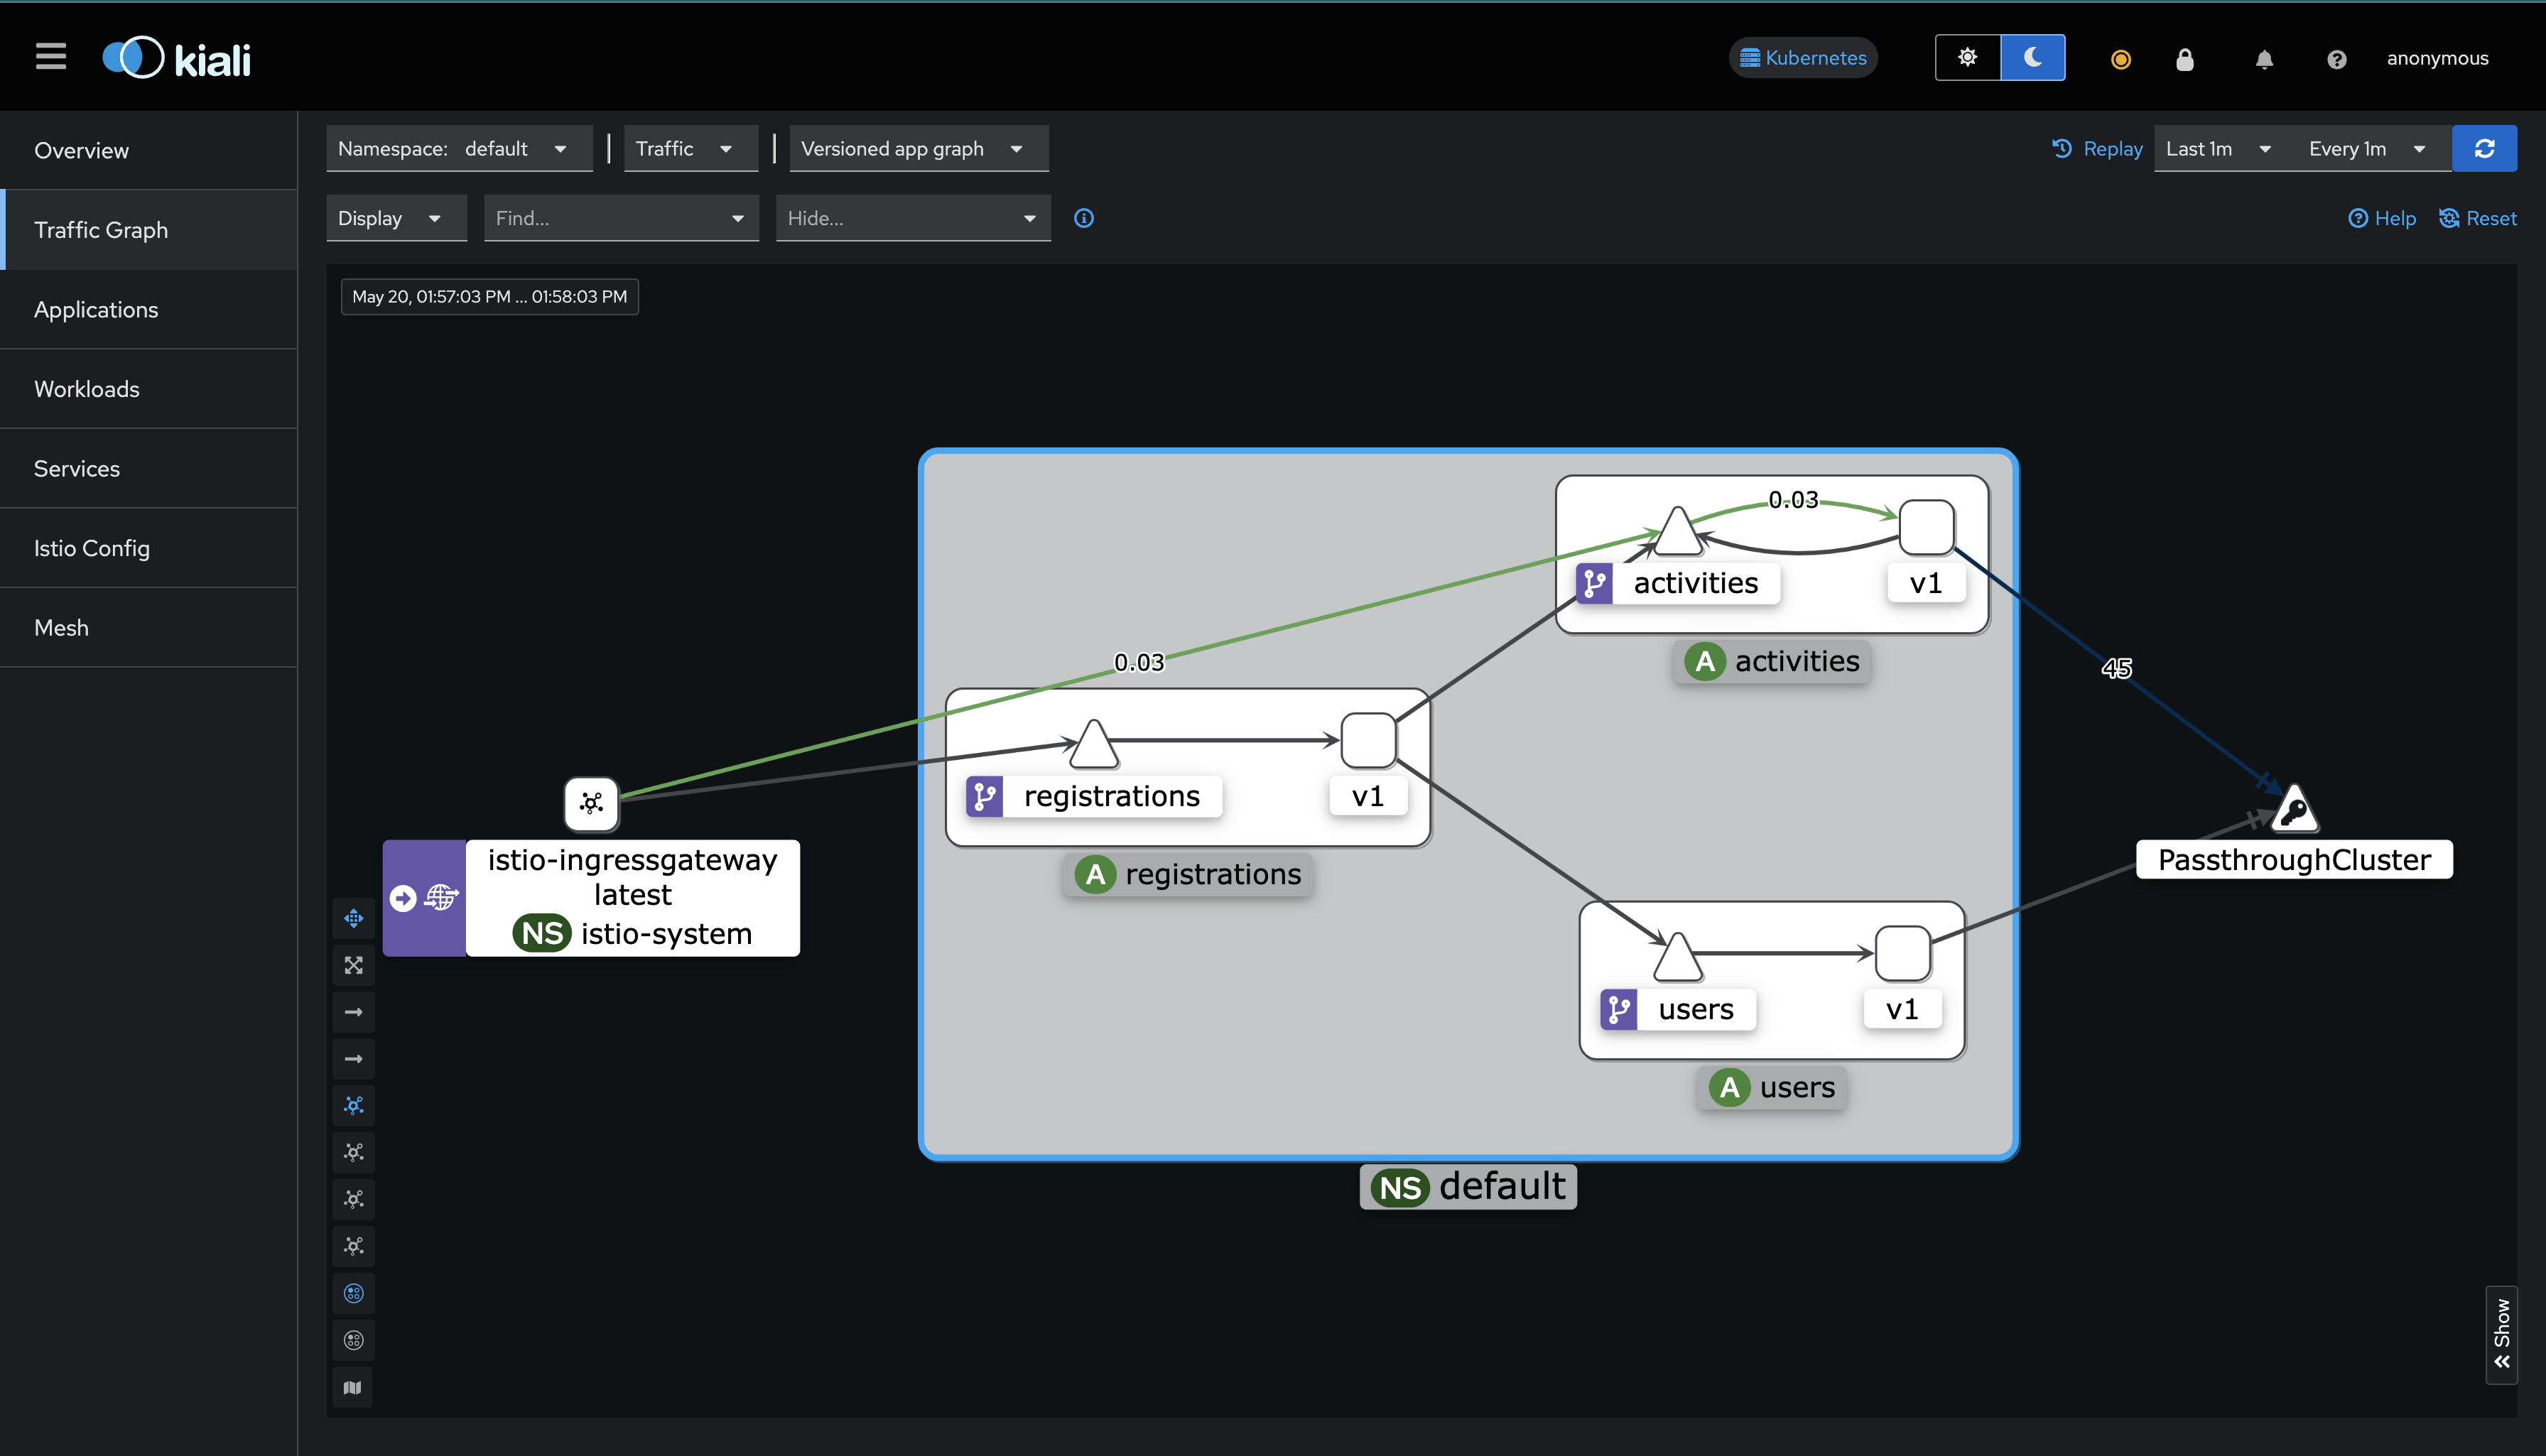
\includegraphics[width = 16cm]{kialiActivity.png} 
    \caption{Kiali Console met verkeer} 
    \label{fig:kaili2}
\end{figure}

Als de activiteit details van de registartieservice worden aangeroepen, roept de registratieservice de activiteitenservice aan. In de Kiali-console wordt dit weergegeven als een verbinding tussen de registratieservice en de activiteitenservice \ref{fig:kaili3}.

\begin{figure}[H]
    \centering	
    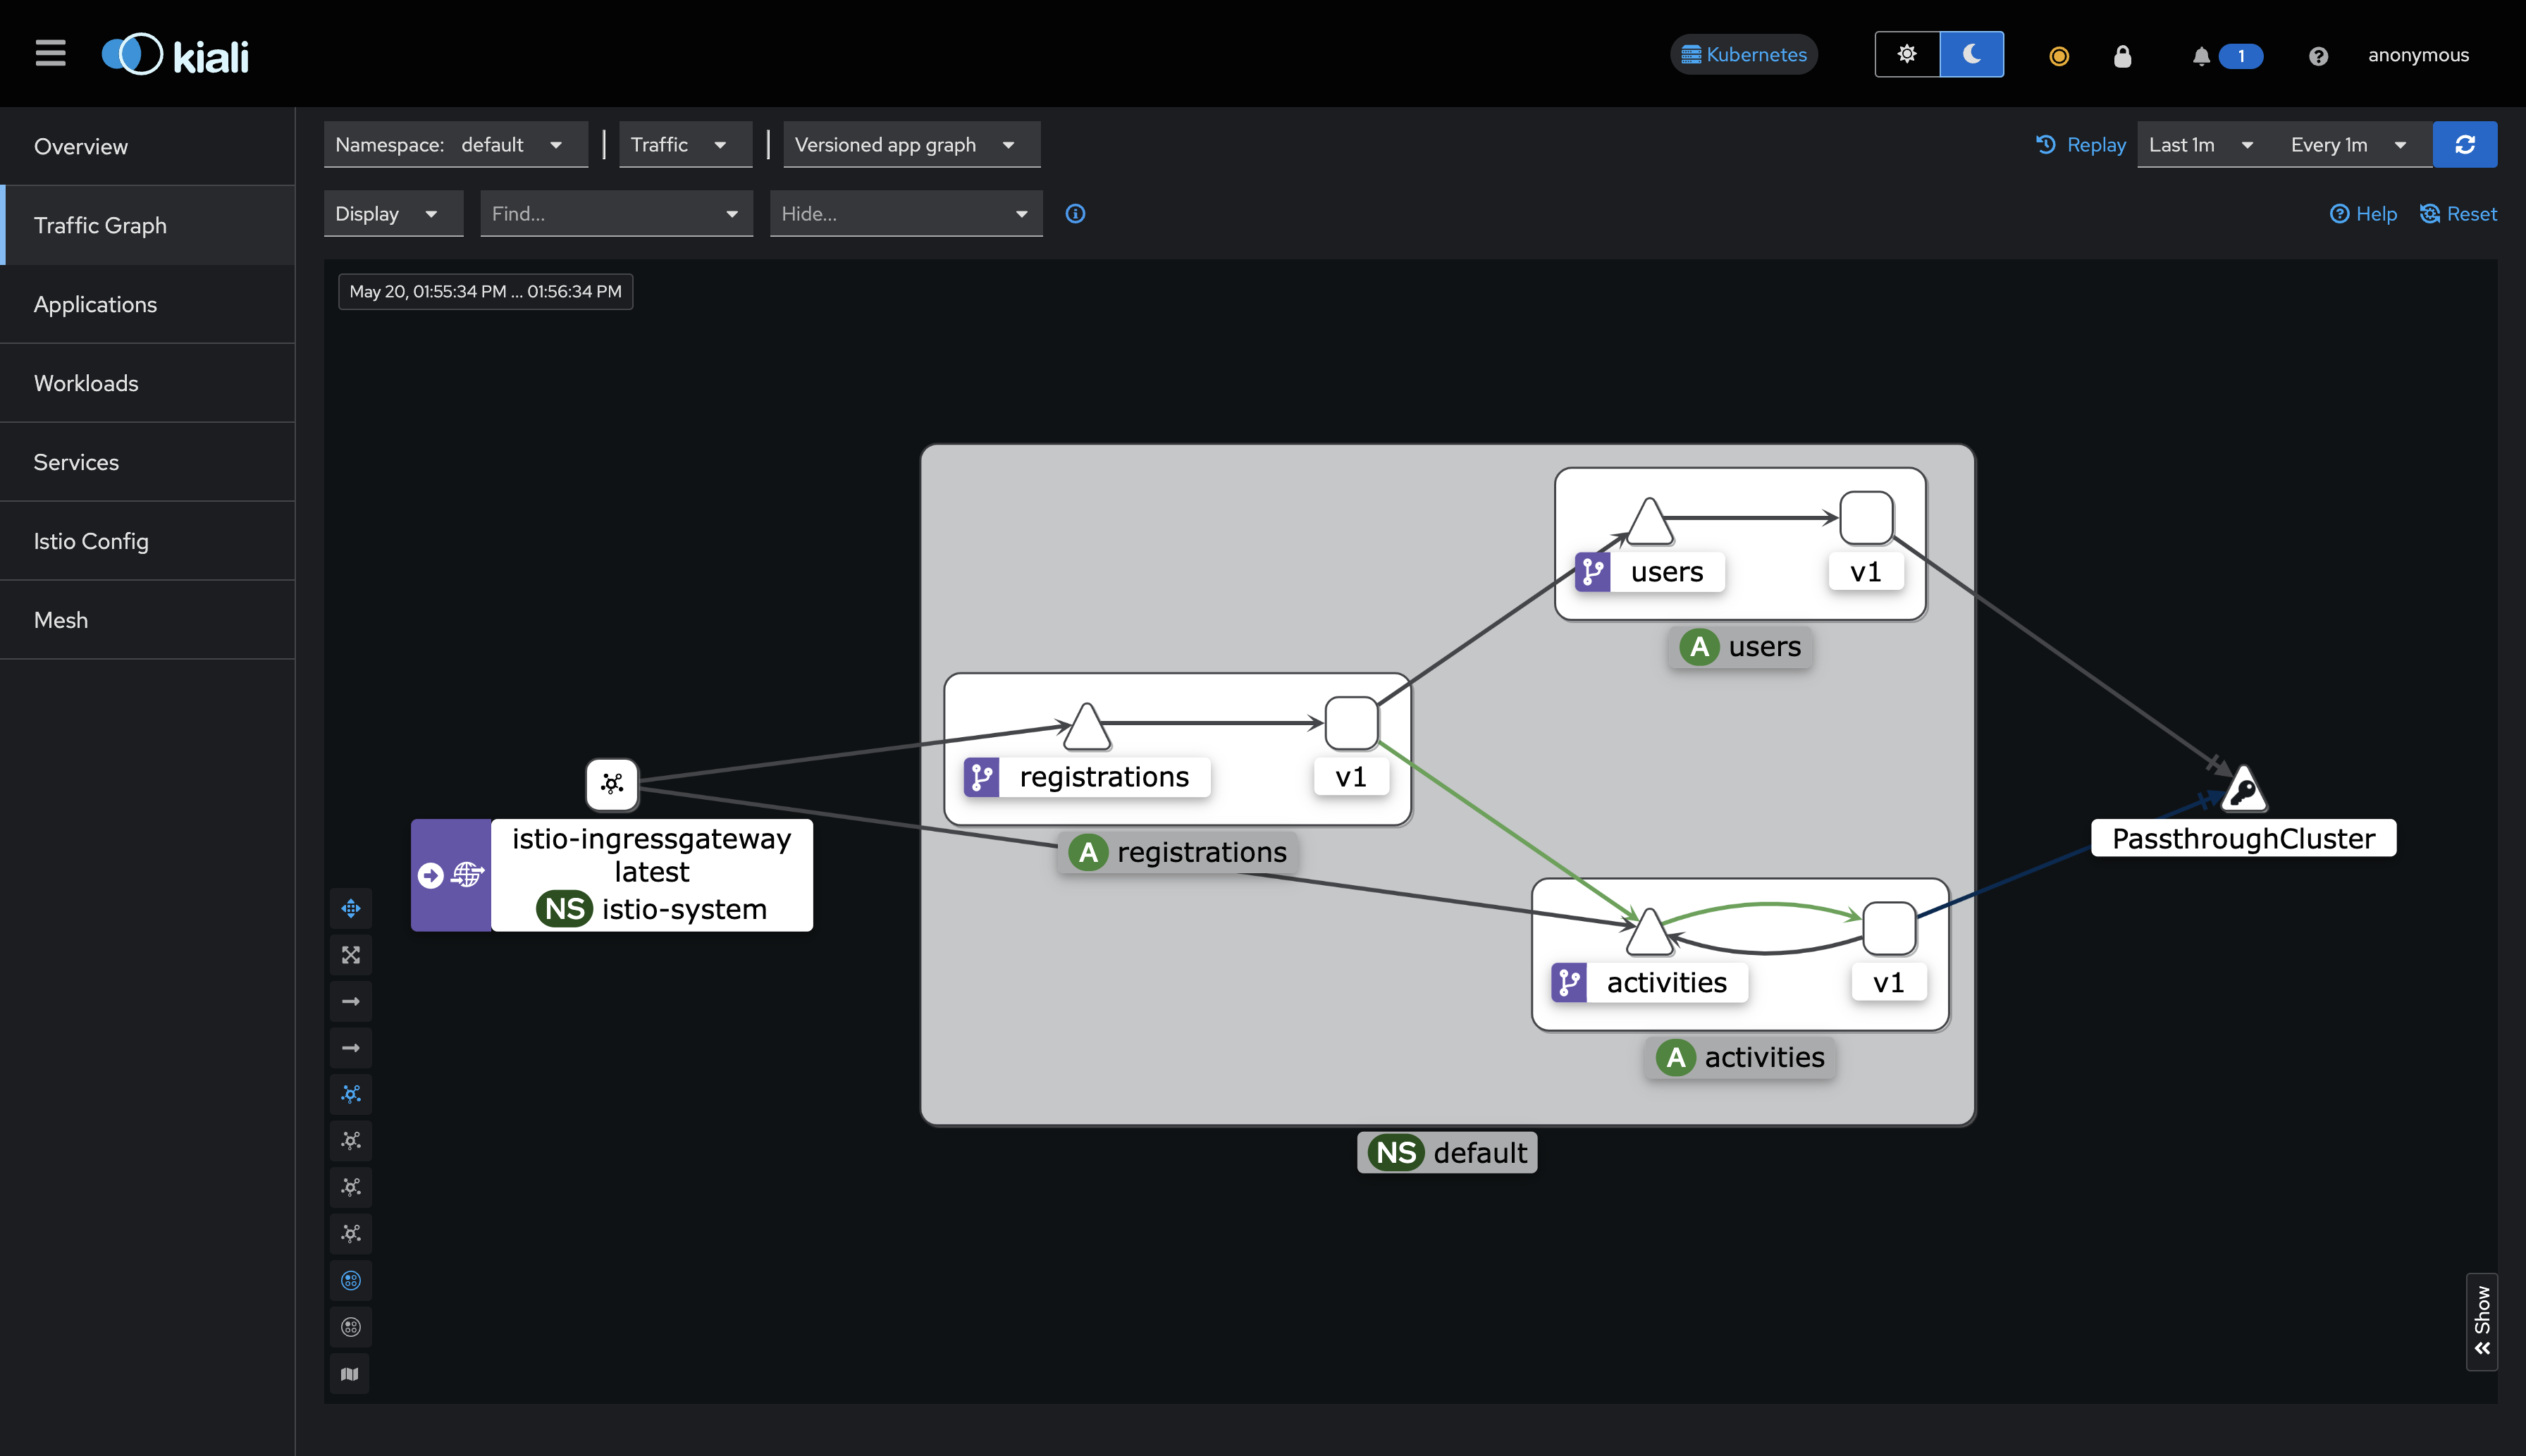
\includegraphics[width = 16cm]{kialiRegistration.png} 
    \caption{Kiali Console met verkeer} 
    \label{fig:kaili3}
\end{figure}

